%! tex root = ../master.tex

\chapter{System Design}
\label{chap:system_design}

In this chapter the project is further analysed. Diagrams are given
and other notions are described, setting up the premise for implementing
\OSname{} based on the \arinc{} standard.

\section{System Overview}
As a means to both explain the system and as a practical development
model, the system can be thought of as being made up of layers.
Each layer being an abstraction of functions in the layers beneath it,
with the partitions at the top and the hardware at the bottom.
The model in figure \ref{fig:simple_system} is defined by the \arinc{} standard
and expanded upon here with drivers being built on top of the HAL library,
instead of directly on top of the hardware, creating an extra layer of
abstraction.

\begin{labeling}{HAL and CMSIS}
	\item [\textbf{Partitions}]
		are independent program units that contain applications. These
		applications can in turn interact with other systems. The
		partitions are achieving this while separated from one another.
	\item [\textbf{APEX}]
		defines the methods by which the partitions talk to other
		modules and
		interact with other partitions or the OS, running
		on the same core module or connected to other ARINC systems.
	\item [\textbf{OS kernel}]
		provides the infrastructure for partitions to operate. This
		includes their scheduling, message passing and processes
		the APEX calls.
	\item [\textbf{Schema}]
		contains the data necessary for the system initialisation.
	\item [\textbf{Drivers}]
		define the way the hardware runs.
		They serve the OS with methods to create an environment in which
		partitions can run and scheduled without influencing one
		another.
	\item [\textbf{HAL and CMSIS}]
		are libraries that provide hardware abstraction layers for
		setting up the hardware.
	\item [\textbf{Hardware}]
		the physical platform on which the OS is executed. This
		includes the CPU and its peripherals.
\end{labeling}

\begin{figure}[H]
\centering
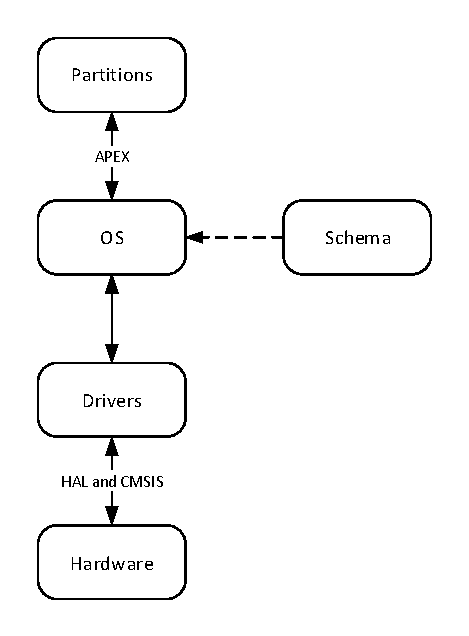
\includegraphics[width=7cm,keepaspectratio]{simple_system_architecture.pdf}
\captionof{figure}{A simple system overview}
\label{fig:simple_system}
\end{figure}


\subsection{Essential components}
\label{design:features}
The rest of the chapter describes the layers of the system from the bottom up.
The hardware specifications are outlined, together with some essential features
needed to make \OSname{} functional and testable as required in chapter
\nameref{chap:Problem_Statement}.
The overall problem being the implementation of an \arinc{} OS,
application execution and control is the end goal.
To facilitate this, the following components must exist:
\begin{itemize}
	\item Hardware platform
	\item Interfaces to interact with the hardware
	\item A program to parse system configurations from a schema to the kernel at compile time
	\item A scheduler for partitions
	\item A scheduler for processes
	\item Partition communication
	\item System calls to handle APEX calls
\end{itemize}

The design of these components is described in the rest of the chapter.
Memory separation is not an essential feature for facilitating the execution of applications,
but is essential to separate them for security and reliability reasons,
thus memory protection is also described.

The features ``Health Monitor'' and ``Intrapartition Communication'' have been
excluded from the project to limit the scope to a manageable amount.


\section{Hardware}
As mentioned in the \nameref{section:settleing_platform} section,
the hardware used for the development of this system is the Mini-M4
board. It is build around the STM32F415RG microcontroller\cite{stm32_datasheet}, based on
an ARM Cortex-M4 core. This is a 32-bit RISC architecture CPU using
the ARMv7M instruction set\cite{arm_architecture}. Additional information
was found in the ARM technical reference\cite{arm_technical}

The chip provides two interfaces for debugging:
%page 1683 reference manual
\begin{itemize}[noitemsep]
	\item JTAG Debug Port (JTAG-DP)
	\item Serial Wire Debug Port (SW-DP)
\end{itemize}
There was no thought process involved in choosing one of the two.
The JTAG interface is enabled by default, and worked right from the
early phases of the project. In some situations, SW would have been
preferred to JTAG, due to physical space constraints. JTAG uses 5
wires, while SW only uses 2. Also, the IDE of choice can have some limitations
on the debugging platform.

JTAG is actually an association\footnote{Joint Test Action Group}
that develops standards about how
physical circuit boards should be tested. However, for the rest of
the document, JTAG will be referred to as the main communication interface
for the Mini-M4 board. This will mainly be used for flashing the program
on the chip and debugging it. In order for a computer to access this
interface, the STLINK-V2 in-circuit debugger/programmer\cite{st_link}
is used, through USB.\\

Another way of communicating with the chip is the serial communication.
For this purpose the UART will be used. This is a common peripheral for
embedded devices, but it needs to be set up before it can be used. This
involves initialising the UART, configuring the data format and the
transmission speed and sending the actual data. In order to see this data
on a computer, one could use a serial-to-USB adapter \cite{ttl_usb}.
This creates a virtual COM (Communication port), that is accessed using
a serial console such as PuTTY\footnote{Free and open-source terminal emulator, serial console and network file transfer application}.
\\\\
The final setup of the Mini-M4 board comprises of the 5 wires from the JTAG,
the 2 wires from the UART, the mini-USB cable that provides power and a
breadboard to accommodate electrical connections.


\section{Memory Map}
\label{sec:memory_map}
The STM32F415RG microcontroller has 1 MB of flash memory. The flash
is non-volatile memory, used for storing programs and
data.\\

There are 192 KB of RAM, divided into 128 KB of SRAM and 64 KB of
CCM data RAM.
The SRAM is volatile memory, where the $static$ tag means
that it does not need to be refreshed in order to
keep its state. This is divided furthermore into a section of 112 KB, and
another of 16 KB, which can be useful if one needs to boot from RAM\cite{run_from_ram}.
They are adjacent in address space and can be treated as one block.
The memory has a feature called bit-banding, in order to let the system
perform atomic operations on bits\cite{bit_banding}.\\

The other 64 KB of CCM data RAM are always ready for access by the CPU,
but cannot be accessed by the peripherals through direct memory access.
Beside the 192 KB of SRAM, there are 4 KB of SRAM used for backup purposes.
These won't be used, since they are not within the scope of the project.\\

Figure \ref{fig:memory_model} presents a simplified model of the
memory map implemented in the STM32F415RG microcontroller\cite{stm32_datasheet_74}.
The blocks on the left column are legacy of the ARM Architecture.
This provides 4 GB of addressable memory.
Some of these regions are correlated to the microcontroller\textquotesingle s
actual memory, as it can be seen in the column on the right. Each block
in this column contains their start and end addresses, on their side.

\begin{figure}[H]
\centering
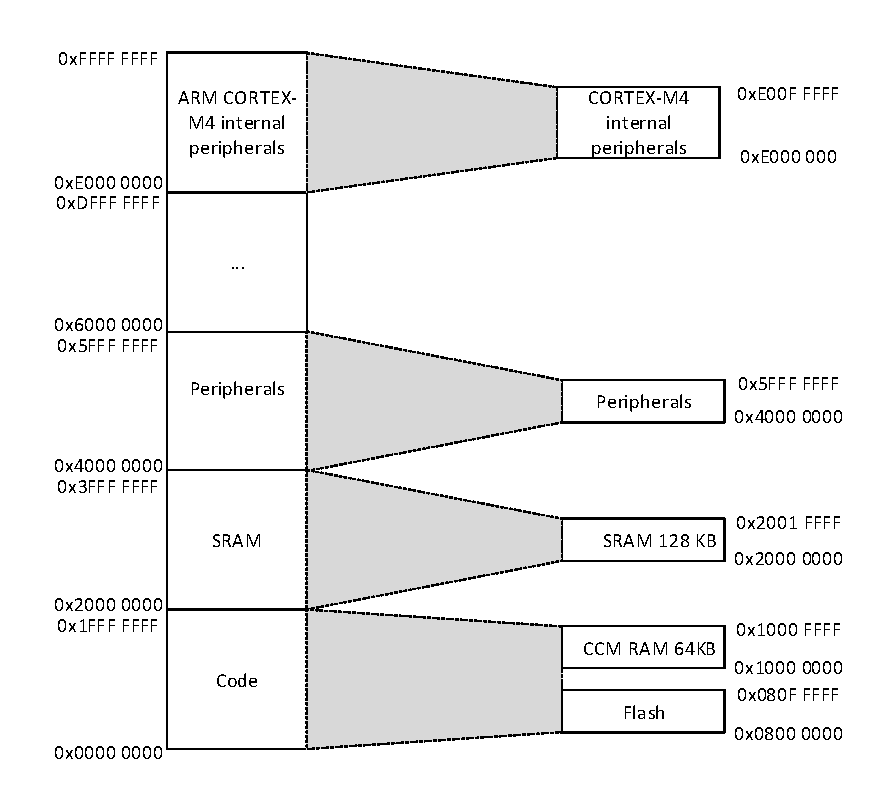
\includegraphics[width=\linewidth,keepaspectratio]{memory_model.pdf}
\captionof{figure}{Memory map}
\label{fig:memory_model}
\end{figure}

The ARM relies on memory mapped IO to communicate with peripherals,
as seen in the upper two blocks of the memory map.

\section{HAL and CMSIS}
These two libraries are the workhorses when dealing with the
board\textquotesingle s peripherals. By using them, the development
process usually has a quick start, removing the steepness of the
learning curve.\\
HAL (Hardware Abstraction Layer) is provided by the chip manufacturer - STMicroelectronics.
The source files are available at their website,
along with its documentation \cite{HAL_library}.
The CMSIS (Cortex Microcontroller Software Interface Standard)
can be seen more as a framework, than a library
 \cite{CMSIS_core_library}. It is provided
by ARM, the company developing the chip architecture.\\

As seen in figure \ref{fig:CMSIS_HAL}, CMSIS
defines the data structures and address mapping for some of the ARM peripherals.
Besides this, it can be used to configure the microcontroller
oscillators, as well as providing support for the instrumentation trace during debug sessions \cite{cmsis_reference}.
The HAL library can then use these definitions for implementing its utilities.
One could easily say that HAL is build on top of CMSIS.
This can be further understood by looking at the way CMSIS handles
the exceptions occurring in the chip, while the HAL library configures
these interrupts.

\begin{figure}[H]
\centering
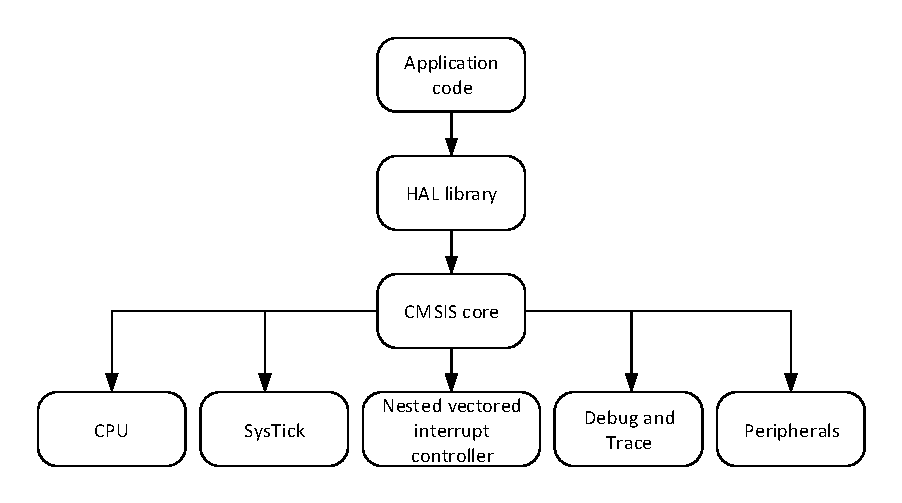
\includegraphics[width=\linewidth,keepaspectratio]{HAL_CMSIS.pdf}
\captionof{figure}{The structure of the libraries (inspired by:
\cite{cmsis_picture})}
\label{fig:CMSIS_HAL}
\end{figure}


\section{Drivers}
The drivers controlling the hardware would have to be implemented at an
early stage of the project, in order to have access to the low level
subsystems.
The following list contains the drivers that would provide the OS a basic
interface to access the hardware.

\begin{labeling}{Watchdog timer}
	\item [\textbf{System Clock}] provides the frequency at which the
	peripherals are synchronised. This can later on be scaled up or down
	to generate the CPU\textquotesingle s and peripherals\textquotesingle
	\ \ clock.
	The system clock relies on an oscillator.
	There is a multitude of choices, ranging from internal or external
	oscillators, to high or low speed crystals. In some cases, certain
	peripherals can use their own, independent clock sources that also have
	to be configured
	\item [\textbf{UART}] used by the system to communicate with the outside
	world. This can either receive or transmit data to another UART devices
	\item [\textbf{LEDs}] mainly used for debugging. They are
	connected to two of the GPIO pins
	\item [\textbf{Delay}] is a simple function, based on calling another
	function from the HAL library. It delays the execution
	of the program by a number of milliseconds. Mainly used for debugging
	\item [\textbf{MPU}] provides the system a way to manage its
	memory. This is required by the ARINC 653 standard.
	Operating systems built on more advanced processors generally use
	an MMU
	\item [\textbf{Timing}] has the purpose of keeping track of
	relative time. As the standard specifies, it should be counting
	nanoseconds
	\item [\textbf{Watchdog timer}] necessary to ensure recovery
	in case of a hardware fault or program error. If this happens, the
	program would be restarted
	\item [\textbf{RTC}] has the purpose of keeping track of
	time accurately. Usually it uses  a 32,768kHz oscillator as a
	clock source, which is the standard in the field
\end{labeling}

These drivers should be implemented as standalone C files. They could then
be used by including their header files where needed and calling their
functions.
The basic functionalities of a driver are:
\begin{itemize}[noitemsep]
	\item initialisation of the peripheral
	\item usage of its resources
	\item de-initialisation (if needed)
\end{itemize}


\section{OS kernel}
The OS kernel has the purpose to link the APEX interface with the hardware.
This is a monolithic kernel. The following sections contain
the kernel\textquotesingle s features and functionalities.


\subsection{Scheduler}
\label{ssec:design_scheduling}
Schedulers are used to allow a system to run more processes than there are
available CPU cores.
A scheduler decides which process to execute by an available processor,
according to predefined rules. Based on these rules, two or
more processes may run concurrently, sharing CPU time. The ARINC 653
specification defines two levels of scheduling, a partitions level scheduler and a
process level scheduler. The algorithms for both are strictly defined.\\

The partition level scheduler uses manual scheduling. Time is split into fixed
length intervals, major frames. Each partition is given one or more windows
(i.e. time slices) in the major frame. Each window has a start time
relative to the time of the major frame and a duration. Windows are set up by
the system integrator in the XML file\cite{arinc_part_scheduling}.
When a partition has run for the duration it is specified, the scheduler will
switch to the partition containing the next window. The switch will happen regardless of
what the partition is doing at that time; a partition can not overrun its
allotted time and thereby cause other partitions to overrun their deadlines.\\

The process level scheduler is a pre-emptive priority scheduler. All processes
will always have a priority. Processes can only be scheduled when the
partition they belong to is scheduled by the partition level scheduler. The
process scheduler selects the process with the highest priority that is also
in the ready state. If two or more processes have the same priority, the one
that became ready first is scheduled\cite{arinc_pro_scheduling}.\\

The ARMv7M architecture has two special interrupts that are especially useful
for scheduling: SysTick interrupt and PendSV interrupt. The SysTick interrupt is
triggered at a regular interval, and can be used for time based scheduling. The
PendSV interrupt is triggered by software and can be used to trigger
scheduling from other interrupt service routines, e.g. when a process blocks to
wait for something.


\subsubsection{Context switching}
Context switching, means switching from executing one block of code $b_1$ to another block of code $b_2$
with the intent to eventually return to $b_1$ in a way that is transparent to the blocks of code.
This allows code to be partitioned into separate independent blocks that can run concurrently.
This is opposed to monolithic blocks of code that entirely control the flow of execution.
Therefore, context switching is essential for any operating system that wishes to utilise a scheduler to allow concurrent execution of code.
Context switching works by saving the state of the CPU registers from one context to memory,
and then switching to another context by restoring the state of the registers previously saved in memory.
Since context switching must manipulate registers directly and individually, it is a feature that must be implemented
on a very low abstraction level, and it can change significantly from one CPU architecture to another.
The scope of this project is to only implement an operating system for a Cortex M4. Hence context switching needs only
to work on the architecture used by this chip.\\

Context Switching on the Cortex M4 is partially handled by the Nested Vectored Interrupt Controller (NVIC).
When an exception (this includes interrupts) occurs, the NVIC will change context to an exception handler.
Upon changing context from regular code to the exception handler, the NVIC will save the registers R0-R3, R12, LR, PC and PSR
on the stack. These are only some of the registers.
When the exception handling routine exits, and control is handed back to the NVIC,
the NVIC will restore these registers again.\\

If the operating system wishes to switch context, it must save the remaining registers, R4-R11, and the stack pointer to memory,
pick a new context to restore, reload the registers R4-R11 and the stack pointer of the new context from memory,
and hand back control to the NVIC. The NVIC will then reload the remaining
registers from the stack of the new context. Table \ref{tab:registers} shows the registers
and who saves them.\\

\begin{table}[H]
	\centering
	\begin{tabular}{|c|c|p{9.5cm}|}
		\hline
		Register	&	Saved by	&	Purpose\\
		\hline
		R0			&	Hardware	&	General purpose (Argument value + return value)\\
		\hline
		R1-R3		&	Hardware	&	General purpose (Argument value)\\
		\hline
		R4-R11		&	Software	&	General purpose (Local variable)\\
		\hline
		R12			&	Hardware	&	General purpose (Intra-Procedure-call scratch)\\
		\hline
		R13 (SP)	&	Software	&	Stack pointer [Banked]\\
		MSP			&	Software	&	Master stack pointer (Stack pointer for kernel space)\\
		PSP			&	Software	&	Process stack pointer (Stack pointer for user space)\\
		\hline
		R14 (LR)	&	Hardware	&	Link register\\
		\hline
		R15 (PC)	&	Hardware	&	Program Counter\\
		\hline
		xPSR		&	Hardware	& 	Special-purpose Program Status Register\\
		\hline
	\end{tabular}
	\captionof{table}{A table of the CPU registers of a Cortex M4. Notice that register R13 (stack pointer) is banked;
	there are separate registers for user space and kernel space.
	For registers, aliases are written in parenthesis, and for purpose, calling convention is written in parenthesis.}
	\label{tab:registers}
\end{table}

Additionally, the Cortex M4 utilises two different stack pointers, the Master Stack Pointer (MSP) and the Process Stack Pointer (PSP).
The MSP is intended for kernel space execution and the PSP is intended for user space execution, but there is no enforcement.
Switching between the two cannot be done in an exception handler, but must instead be done by the NVIC.
Since the path to the new context goes through the NVIC, the NVIC is also partially responsible setting the state of the processor.
This is done by loading an EXC\_RETURN value into the Program Counter. See table \ref{tab:exc-return} for the different EXC\_RETURN values.
To make context switching transparent to the applications running, it is important that the state the processor returns to, is the
same it came from earlier. Therefore, upon entry into the interrupt routine, the NVIC loads the appropriate EXC\_RETURN into the Link.
This value must be saved by software to assure it can return to the right state.

\begin{table}[H]
	\centering
	\begin{tabular}{|c|p{10cm}|}
		\hline
		Value			&	Description 	\\
		\hline
		0xFFFF FFF1 	&	Return to Handler mode, using the Master Stack Pointer, but without the floating point unit.	\\
		\hline
		0xFFFF FFF9		&	Return to Thread mode, using the Master Stack Pointer, but without the floating point unit.		\\
		\hline
		0xFFFF FFFD		&	Return to Thread mode, using the Process Stack Pointer, but without the floating point unit.	\\
		\hline
		0xFFFF FFE1		&	Return to Handler mode, using the Master Stack Pointer, with the floating point unit.			\\
		\hline
		0xFFFF FFE9		&	Return to Thread mode, using the Master Stack Pointer, with the floating point unit.			\\
		\hline
		0xFFFF FFED		&	Return to Thread mode, using the Process Stack Pointer, with the floating point unit.			\\
		\hline
	\end{tabular}
	\captionof{table}{
		A table of the possible EXC\_RETURN values. An interrupt service routine
		is exited by loading one of these values into the Program Counter register.}
	\label{tab:exc-return}
\end{table}


\subsection{Interpartition communication}
\label{design:interpart_comm}
Interpartition communication as introduced in section \ref{ssec:interpart_comm}, is a basic mechanism for linking partitions by messages using channels.
Each partition can be linked to multiple channels by ports.
A partition can interact with its ports by using the APEX to send or receive messages.\\

At the application level messages are atomic and as such channels are required to ensure the correctness of every message received\cite{arinc_interpartition_comm_atomic}.
Multiple different modes exist for the messages and different checks and methods should be applied to comply with the ARINC 653 standard.
Only a subset of these features is designed and implemented,
to give a basic feature set which allows partitions to communicate on a single microcontroller.\\

A simplified design of queuing ports and sampling ports is made for \OSname.\\

Since ports and their attributes are declared and defined statically,
very little has to be done to initialise them at startup.
Ports are organised as belonging to some partition and channel.
They have attributes according to their port type, as well as common attributes:

\begin{itemize}
	\item The port name
	\item A flag indicating the port type
	\item A port direction indicating whether the port is a destination or a source
	\item Maximum message size
	\item A reference to the channel it belongs to
\end{itemize}


%A port can be viewed as belonging to some partition,
%hence ports can be structured in multiple arrays,
%with each array containing the ports belonging to a particular partition.
%This way of structuring results in every port having to contain a reference to its channel,
%as stated in the above list.

A port belongs to a partition and contains a reference to its channel.
Some necessary attributes for queuing ports and sampling ports are listed in
the sections \ref{sssec:queuing_ports} and \ref{sssec:sampling_ports} respectively.


\subsubsection{Queuing Ports}
\label{sssec:queuing_ports}
The necessary attributes for queuing ports are the following:
\begin{itemize}
	\item Number of messages received in the queue
	\item Maximum number of messages to be held by the receive buffer
	\item A circular buffer to act as the FIFO buffer
\end{itemize}

The OS has to facilitate some methods to push and pop complete messages to and from a circular buffer,
which would be auto-generated from the configuration file.
\OSname\ also has to provide functions to handle the following APEX calls defined in the standard\cite{arinc_interpartition_comm}:

\begin{itemize}
	\item CREATE\_QUEUING\_PORT
	\item SEND\_QUEUING\_MESSAGE
	\item RECEIVE\_QUEUING\_MESSAGE
	\item GET\_QUEUING\_PORT\_ID
	\item GET\_QUEUING\_PORT\_STATUS
\end{itemize}


\subsubsection{Sampling Ports}
\label{sssec:sampling_ports}
The attributes for sampling ports are the following:
\begin{itemize}
	\item A refresh period time
	\item An indicator for the validity of the last received message
	\item A buffer to hold the sampling message
\end{itemize}

The OS has to facilitate some methods to transmit and validate sampling messages.
A simple buffer has to be provided for this by the auto-generated structures.
\OSname\ also has to provide functions to handle the following APEX calls defined in the standard\cite{arinc_interpartition_comm}:

\begin{itemize}
	\item CREATE\_SAMPLING\_PORT
	\item WRITE\_SAMPLING\_MESSAGE
	\item READ\_SAMPLING\_MESSAGE
	\item GET\_SAMPLING\_PORT\_ID
	\item GET\_SAMPLING\_PORT\_STATUS
\end{itemize}


\subsection{Memory Management}
ARINC 653 advertises time and space separation covered in.
\todo[inline]{ref to sec in analysis}
To accommodate for the feature of separating partitions in space,
this operating system relies on the memory protection unit (MPU)
to manage permissions across sections of memory,
ensuring that partitions stay within a dedicated memory space.\\

Dynamic memory allocation is not permitted at runtime
outside predefined memory sections.
This policy ensures a fixed and predictable sandboxed environment, where partitions can not restrict other parts of the system by occupying memory resources.
It also gives the system developer a way to ensure that the system has enough memory for all processes to function correctly, given that this amount is define in the configuration file.

% This figure should NOT be placed near a pagebreak.
% Otherwise it fucks everything up!
% If thats not okay, use normal figure instead.

Memory regions are declared in the configuration file and included at compile time,
as a list of different system features, like individual partitions and communication buffers.
The rest of this section will deal with the subject of managing memory regions on a
STM32F415 chip and categorising and analysing the memory requirements into a single
memory strategy to implement.


\subsection{The MPU on a STM32F415}
\label{ssec:design_mpu}
The MPU can be used to prohibit partitions from corrupting data used by kernel code and other partitions.
The MPU can protect up to eight memory regions and is unified, meaning that it does not distinguish between code and data sections.
Regions can have sub-regions, but because the minimum regions/sub-regions size is the length of a cache line (32 bytes),
sub-regions are only available for regions of at least 256 bytes of size.
Partitions above this threshold can have eight sub-regions.

\begin{wrapfigure}{R}{0.3\textwidth}
	\vspace{-20pt}
	\centering
	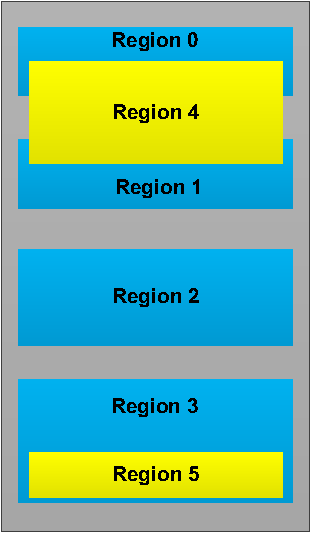
\includegraphics[width=0.3\textwidth]{mpu_overlapping_regions.pdf}
	\caption{Example of nested and overlapping regions from \cite{stm32_mpu}.}
	\label{fig:stm32_mpu}
	\vspace{-40pt}
\end{wrapfigure}

Every region has a fixed priority and is numbered from 0-7, where region 7 has the highest priority.
Regions can be nested and overlapping.
The behavior when nesting and overlapping is dictated by the priority of the region as depicted in figure \ref{fig:stm32_mpu}.


\subsection{Memory strategy}
As the memory available is not abundant, there is the need of avoiding wasting memory.
For that, the memory needed by the partitions is optimised by a sorting algorithm in order to fit
the most partitions possible in a limited region of memory and by expanding the partition size,
fulfilling the empty gaps.
It is important to keep the size,
initial pointer and the region of each partition for enabling and disabling the right area of memory when a different partition is active.


\subsection{System calls}
\label{ssec:design_system_calls}
To improve security and robustness, many modern operating systems make clear
distinctions between the kernel and applications, and they restrict application
code from accessing certain peripheral hardware (e.g. storage devices, I/O
devices) as well as control registers of the CPU.
To restrict only certain code from certain features require hardware support.
To accomplish this, many modern CPUs contain two or more different execution
levels. Normally, the kernel will run in the most privileged execution level
while application code runs in a more restricted execution level. This prevents
application code from changing the state of any resources shared with other
applications. This is critical to accomplish ARINC 653\textquotesingle{}s strict space and time
separation. If partition level code is not run in an unprivileged mode, it will
be able to change the CPU time and memory space allocated to it. However,
since partition level code does on occasion need access to some shared resources,
yet is unable to do so directly, it must request the kernel do it. To do this,
partition level code must preload the general purpose CPU registers, and if
necessary the stack, with a value to identify what the partition wishes the
kernel to do, as well as call arguments, then generate an interrupt which will be
caught by the kernel. Based on the content of the general purpose CPU registers
and the stack, the kernel determines what the partition level code requested,
executes the necessary functions and returns the result in the general purpose
CPU registers and the stack.


\subsection{Error Handling}
The error handler is designed to give the developers the possibility
to see that something has gone wrong in the system.
Since the health monitor is not going to be implemented,
this is the extend to which the error handler is designed.
The idea is to capture only
some of the faults or failures and throw an exception that the error
handler would then catch.

%The error handler is designed in the context of the
%Health Monitor function specified in the standard.
%However, its functionality and specific APEX calls won\textquotesingle t be
%approached, since the goal is only to give the developers the possibility
%to see that something is wrong in the system. The idea is to capture only
%some of the faults or failures and throw an exception that the error
%handler would then catch.


\section{Schema}
\label{sec:design_schema}
An ARINC 653 schema specifies the structure
of the configuration and the required elements
for the core module.
The schema is a recipe used to create a configuration file.


\subsection{Schema design}
The schema defined in figure \ref{fig:open653schema} is not the complete
ARINC 653 schema, though it can be extended
into the full schema with some more work.
%but the subset defined to accommodate the features of open653.
The scope was limited as outlined in the
problem statement \nameref{chap:Problem_Statement}.

\begin{figure}[H]	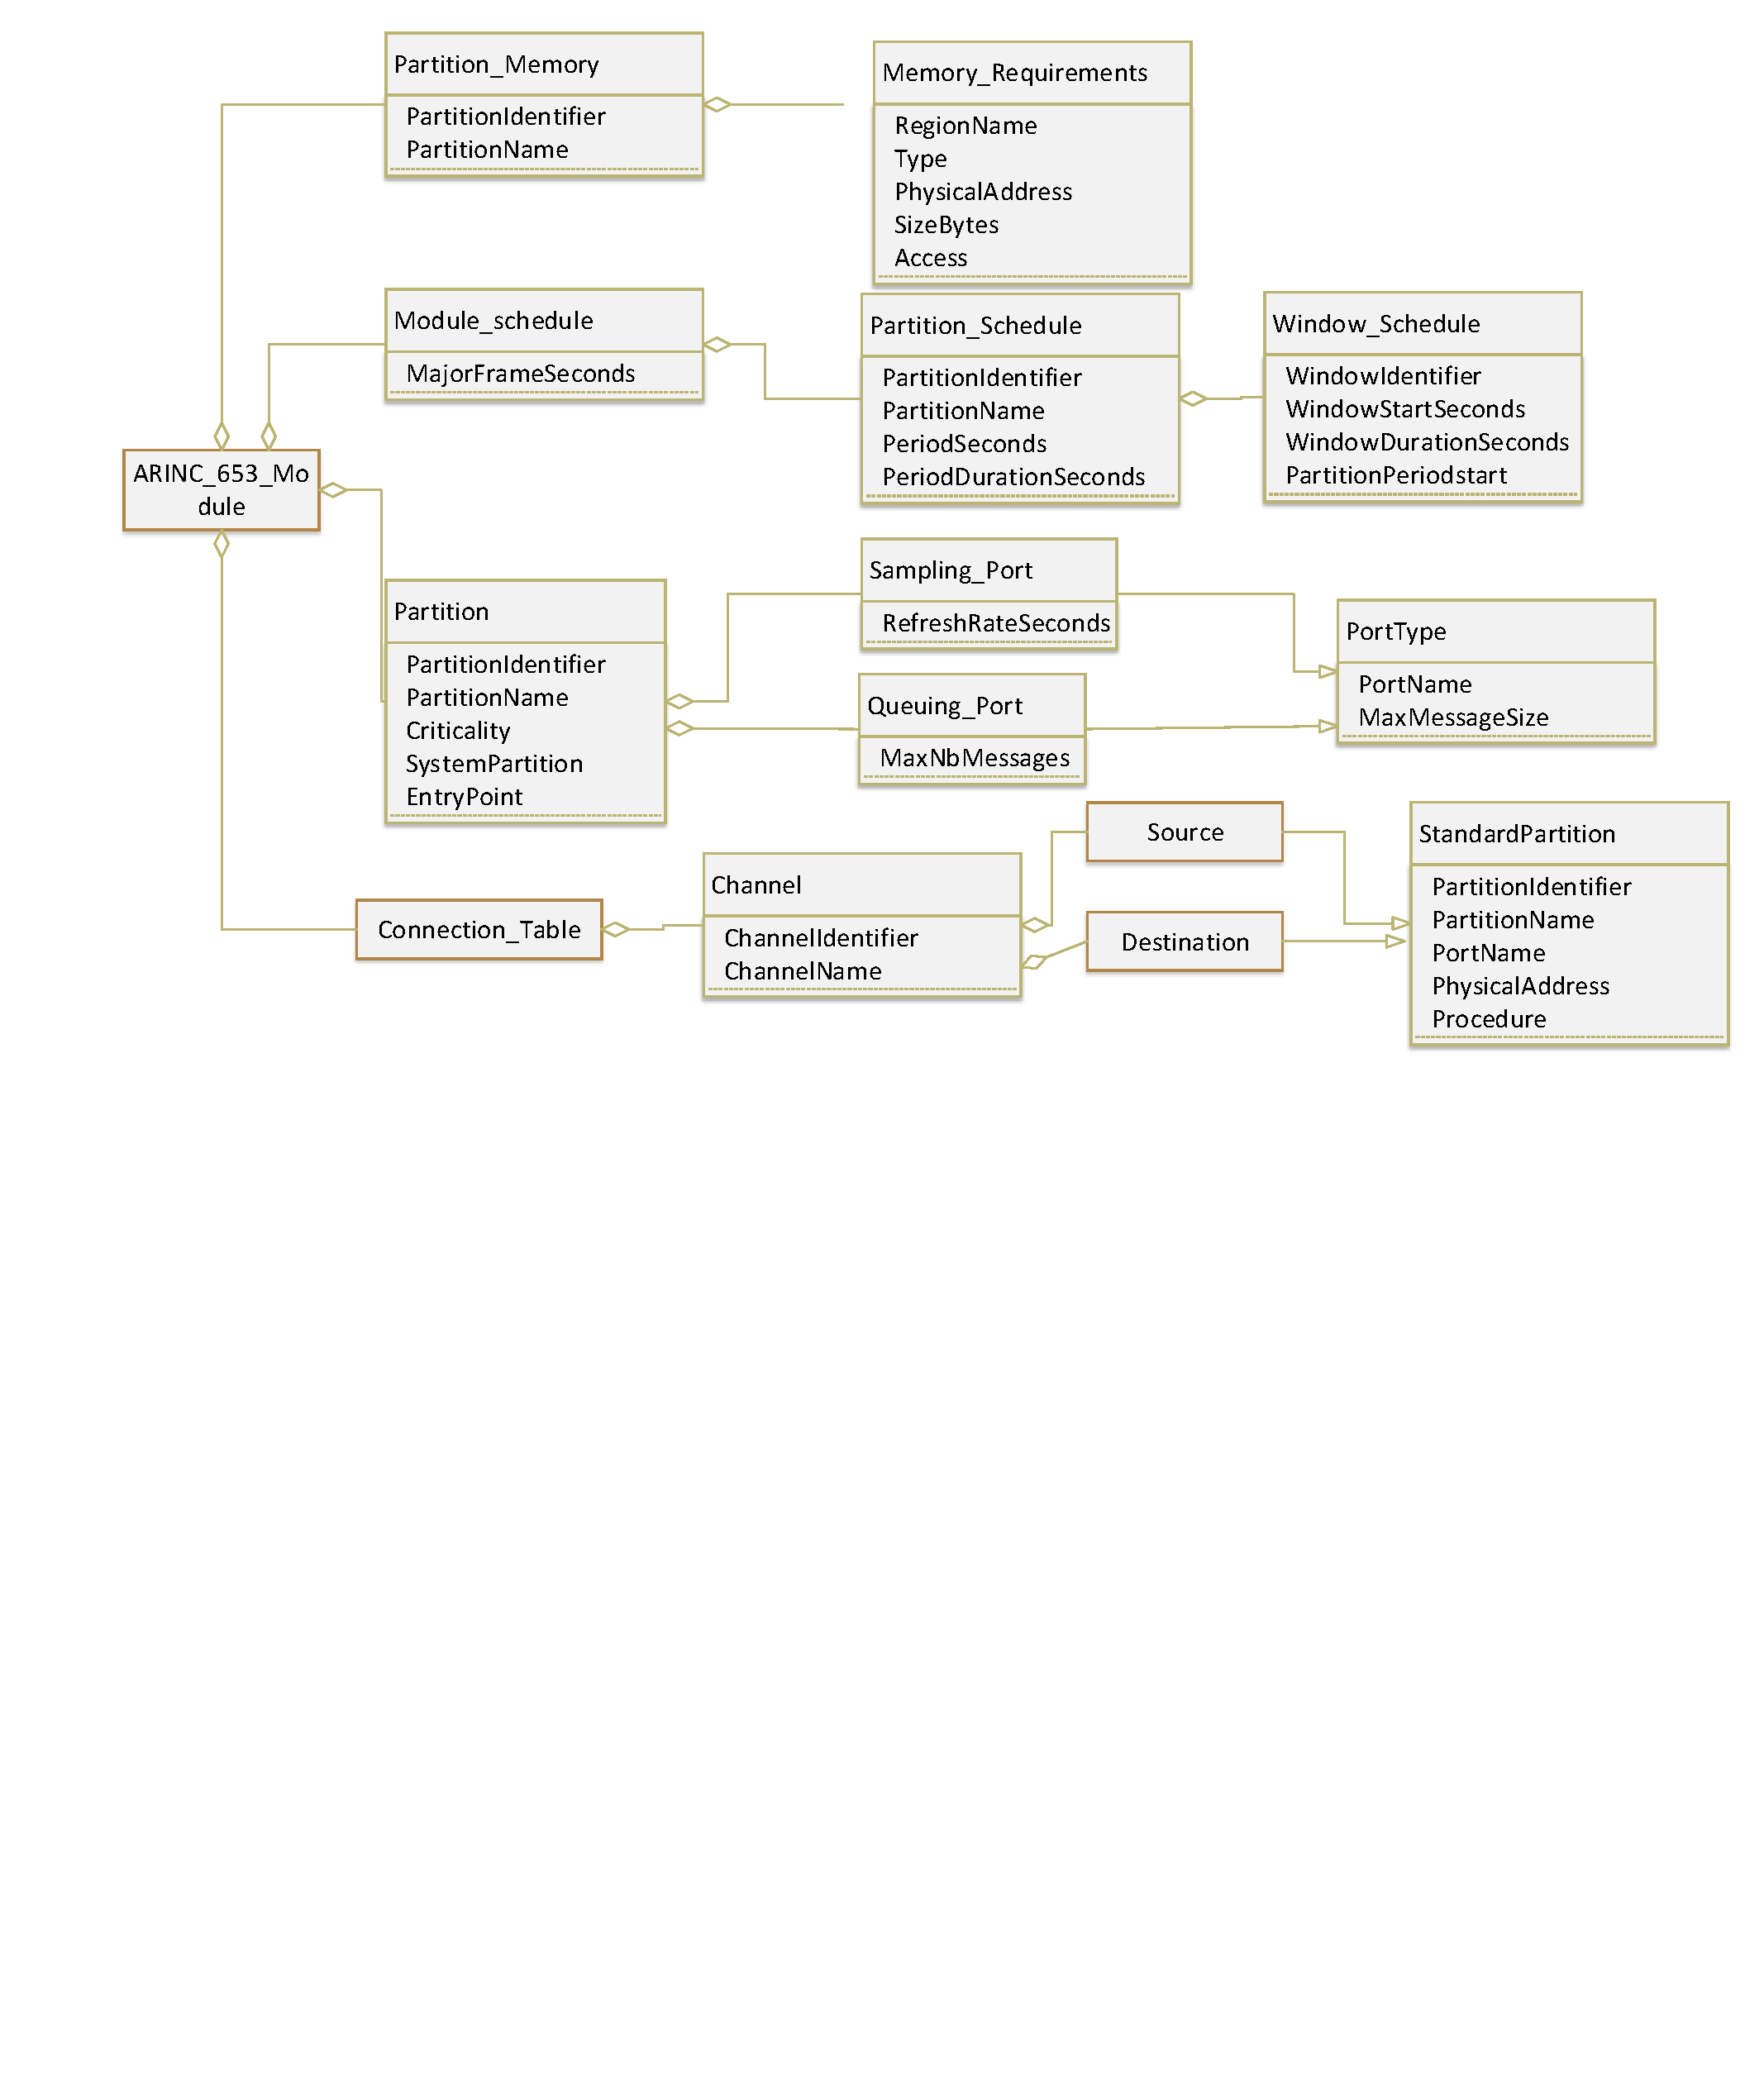
\includegraphics[clip=true,trim=0cm 20cm 0cm 0cm,width=\linewidth,keepaspectratio]{figures/open653schema.pdf}
	\caption{\OSname\ schema design}
	\label{fig:open653schema}
\end{figure}

The figure presents the schema and the
relationship between the elements.
An ARINC 653 Module has four elements.
One or more Partition Memory elements,
a Module Schedule, one or more Partitions and a Connection Table.
\\\\
A Partition\_Memory has one or more
Memory\_Requirements and two attributes which correlate
to its associated partition. The Memory\_Requirements
specify the configuration of Partition\_Memory;
the configuration includes the amount of memory it requires,
the type of data stored, how the data is accessed
and its physical address on the hardware.
\\\\
A Module\_Schedule has one or more
Partition\_Schedules and one attribute which defines
the major frame. The major frame is the smallest
amount of time possible to allow every partition to
run at least once.
\\\\
Partition\_Schedule has one or
more Window\_Schedule and four attributes which correlate
to its associated partition, and defines some timing details
not used in this project. PeriodSeconds and PeriodDurationSeconds
specify the maximum time a partition can use in one cycle for
its Window\_Schedule to complete. These two attributes are unused currently, as
there is not appropriate error handling to make use of it and
Window\_Schedule attributes are sufficient for scheduling.
\\\\
Window\_Schedule defines when a partition needs to run and
for how long it will run. PartitionPeriodStart is not used,
and it purpose is not understood.
\\\\
Partition has one or more queuing ports and one or more
sampling ports; it has five attributes which specify
information about the partition. EntryPoint is the name
of the partition initialisation function, SystemPartition
specifies what type the partition is. Criticality is not
currently used, it is meant to define the importance of a
partition.
\\\\
The ports have four attributes which define information
about the port such as size and source or destination.
Sampling\_Ports are not well supported currently in the
project but will function. This is due to not having or
needing any sampling ports in the current implementation.
\\\\
A Connection\_Table has one or more Channels and zero attributes.
A Channel has one or more source and destination channels and two
attributes which identify the channel. The Source and
Destination have four attributes which correlate
to its associated partition, and define the physical address
of the channel.
\OSname{} is missing an attribute called procedure from Channel,
which is defined in the original \arinc{} schema.
Procedure is meant to be used by ports to interact with drivers.


\subsection{Full ARINC 653 schema}

\begin{figure}[H]
	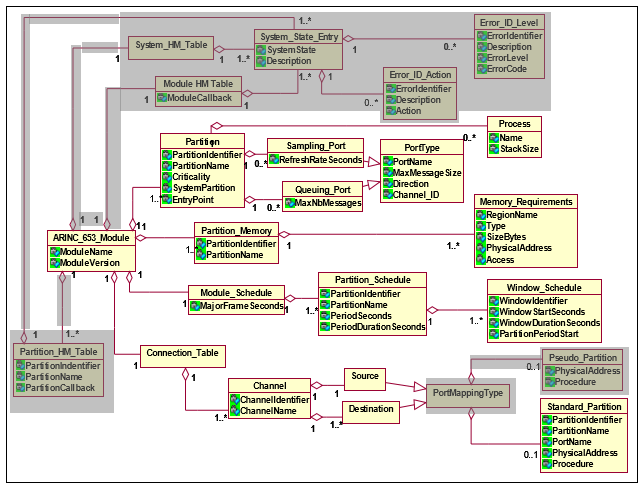
\includegraphics{figures/originalschema.png}
	\caption{full ARINC 653 schema}
	\label{fig:arinc653schema}
\end{figure}

\todo{add ARINC standard reference, grey out unused attributes on diagram}
The figure shows the intended schema for a fully compliant ARINC 653 implementation
as found in the \arinc{} standard. The greyed out areas,
are the aspects of the \OSname{} schema not yet implemented in this project.


\subsection{Schema translation}
XML is the chosen configuration file format.
XML was chosen as opposed to alternatives due to its easy to read and write nature,
\arinc{}\textquotesingle{}s XML example providing guidance and previous experience with XML in the project group.


\section{APEX}
\todo[inline]{needs a reference to the System calls just above, or maybe join them}
The APEX defines an API for applications running on \OSname{}.
Its functions are grouped into
seven major categories \cite{arinc_page_45}. Table \ref{tab:apex_calls}
contains the headers declaring these calls (column on the right),
classified according to the standard.

\begin{table}[H]

	\centering
	\begin{tabular}{|c|p{3.1cm}|}
		\hline
		Category			&	Header file	\\
		\hline
		Partition management 	&	apex\_partition.h	\\
		\hline
		Process Management	&	apex\_process.h\\
		\hline
		Time management	&	apex\_time.h\\
		\hline
		Memory management	&	\textit{No APEX calls}\\
		\hline
	\multirow{2}{*}{Interpartition communication}	&	apex\_sampling.h\\
											& 	apex\_queuing.h\\
		\hline
	\multirow{4}{*}{Intrapartition communication}	&	apex\_buffer.h		\\
											& 	apex\_blackboard.h	\\
											& 	apex\_semaphore.h \\
											& 	apex\_event.h	\\
		\hline
		Health monitoring	& 	apex\_error.h\\
		\hline
	\end{tabular}
	\captionof{table}{
		APEX calls}
	\label{tab:apex_calls}
\end{table}

These header files only declare the calls, which will be implemented later
in the kernel. \textit{apex\_types.h} declares their arguments:
global and
constant variables, as well as the types used by the calls. All the content is found
in the standard, in the form of an ANSI C compliant code.
The input (IN) arguments are types defined here. The output (OUT)
arguments are dependent on the \texttt{RETURN\_CODE} value.
This can be one of the values shown in listing \ref{lst:apex_types}.

\begin{figure}[H]
\lstset{
	language=C,
	basicstyle=\footnotesize,
	showspaces=false,
	showtabs=false,
	showstringspaces=false,
	tabsize=4,
	breaklines=true
}
\begin{lstlisting}[
	firstnumber=67,
	label=lst:apex_types,
	caption=\textit{apex\_types.h}]
typedef
    enum {
        NO_ERROR       = 0, /* request valid and operation performed    */
        NO_ACTION      = 1, /* status of system unaffected by request   */
        NOT_AVAILABLE  = 2, /* resource required by request unavailable */
        INVALID_PARAM  = 3, /* invalid parameter specified in request   */
        INVALID_CONFIG = 4, /* parameter incompatible with configuration*/
        INVALID_MODE   = 5, /* request incompatible with current mode   */
        TIMED_OUT      = 6  /* time-out tied up with request has expired*/
    } RETURN_CODE_TYPE;
\end{lstlisting}
\end{figure}


\section{Partitions and processes}
\label{design:part_proc}
Partitions as described in \ref{anal:arinc} are defined at compile-time and
contain one or more processes, which are initialised during run-time.
A partition is defined to be one or more structures containing information about
its execution and resources.
As described in the \nameref{sec:design_schema} section, there are multiple
groups of information about each partition. It makes sense to separate this information for
different parts of the system (e.g. only the scheduler needs to know about a
partitions\textquotesingle{} execution window information).\\

While information about the overall partition is defined statically, its
processes are defined and created at runtime and for this reason every partition needs
some memory allocated to store this information. A starting process is created
by default using the partitions\textquotesingle{} entry-point, which is then allowed to
spawn any additional processes.\\

Processes, just like partitions are collections of information. Processes hold
information about their own state and how they are to be scheduled.


\iffalse
\section{Agile development}
The software development process flowed naturally due to previous
experience, curiosity and personal interests. The nature of the project
allowed the team to cover different areas at the same time, while still
doing progress, without having a strict plan. Seen as a whole, the project
was pursued by applying the principles of agile software development.
\todo[inline,color=green]{Maybe move this section somewhere else.}
\fi
\section{Discussion}

Figure \ref{fig:advanced_system} presents the system in its entirety,
with all the components organised in the corresponding layers.

\begin{figure}[H]
\centering
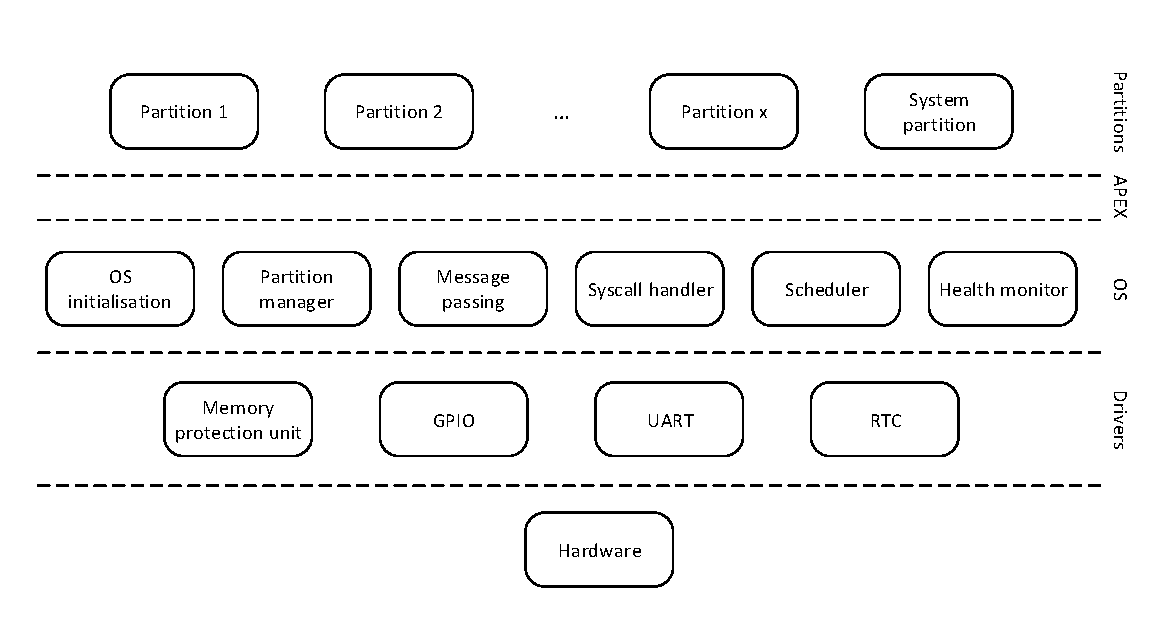
\includegraphics[width=\textwidth]{advanced_system_architecture.pdf}

\caption{An advanced system overview}
\label{fig:advanced_system}
\end{figure}

The following chapter will go through how all these components,
features and functionalities has been implemented.
